\documentclass[11pt]{article}

\usepackage[margin=1in]{geometry}
\usepackage{fontspec}
\setmainfont{Times New Roman}[
  Path=/System/Library/Fonts/Supplemental/,
  UprightFont=Times New Roman.ttf,
  BoldFont=Times New Roman Bold.ttf,
  ItalicFont=Times New Roman Italic.ttf,
  BoldItalicFont=Times New Roman Bold Italic.ttf
]
\usepackage{microtype}
\usepackage{setspace}
\onehalfspacing
\usepackage{amsmath,amssymb,mathtools,bm}
\usepackage{booktabs,threeparttable,array,tabularx}
\usepackage{graphicx}
\usepackage{float}
\usepackage{enumitem}
\usepackage{natbib}
\usepackage[hidelinks]{hyperref}
\usepackage[capitalize,noabbrev]{cleveref}
\usepackage{xcolor}
\usepackage{caption}

\newcommand{\E}{\mathbb{E}}
\newcommand{\Var}{\operatorname{Var}}
\newcommand{\Prob}{\mathbb{P}}
\newcommand{\TV}{\operatorname{TV}}
\newcommand{\RPS}{\operatorname{RPS}}
\newcommand{\LLM}{\textsc{LLM}}
\newcommand{\HGB}{\textsc{HGB}}

\title{\textbf{Synthetic Respondents Without Ambivalence?}\\
\large A Population-Fidelity Audit of Qwen3.5-9B and Machine-Learning Reconstructions of Gender Attitudes in China}
\author{Song Ge\\
\small Wuhan University}
\date{\today}

\begin{document}
\maketitle

\begin{abstract}
Large language models are increasingly used to simulate survey respondents, yet matching a plausible individual answer is not equivalent to recovering a population. This paper evaluates whether a locally deployed Qwen3.5-9B model can reproduce the marginal distributions, heterogeneity, and item structure of five gender-attitude questions in the Chinese General Social Survey (CGSS) 2012, 2018, and 2021. The design pairs 300 real respondent profiles with repeated zero-shot responses and compares them with matched human answers, the full weighted survey benchmark, and survey-trained machine-learning models using the same prediction-time attributes. Qwen3.5-9B produces large item-specific mean errors. Its mean marginal variance ratio is 0.794, but 68.2\% of predictive variance comes from repeated draws within the same profile; the between-profile ratio is only 0.265. A joint five-item prompt also strengthens the housework item's association with the other attitudes. Stateless single-item calls reduce mean absolute correlation by 0.130 (profile-bootstrap 95\% interval: 0.050 to 0.178), although the effect is concentrated in 2018 and independent presentation does not consistently recover the human structure. Histogram gradient boosting remains imperfect for individuals but reduces ordinal MAE from 1.175 to 0.921 and total variation from 0.282 to 0.071. Sparse profiles are therefore a real information limit, but not a sufficient explanation for this model's population distortion.
\end{abstract}

\noindent\textbf{Keywords:} synthetic respondents; large language models; machine learning; public opinion; gender attitudes; China

\section{Introduction}

A synthetic survey respondent can sound plausible without representing any population that exists. A language model asked to speak as a 45-year-old urban Chinese woman with a university education may produce an internally coherent answer to a gender-attitude question. The harder question is whether repeated answers from many such personas reproduce the distribution, heterogeneity, and relational structure observed among comparable people. For social science, these are not secondary properties. Population research depends on variation across respondents, covariance among attitudes, and differences between social groups, not only on whether a single response reads naturally.

Recent work has offered both optimistic and skeptical assessments of large language models as simulated respondents. \citet{argyle2023one} introduce the idea of ``algorithmic fidelity,'' arguing that demographic conditioning can recover complex patterns in human opinion. \citet{aher2023simulate} similarly show that language models can replicate several established experimental findings, although they also identify systematic distortions. Other studies find substantial demographic misalignment \citep{santurkar2023opinions} and warn that synthetic samples can reproduce means while compressing variance, changing regression coefficients, and responding sharply to prompt or model updates \citep{bisbee2024synthetic}. This debate leaves two problems unresolved. First, much evaluation concerns broad American political attitudes, where average alignment can conceal failures in the internal structure of beliefs. Second, when persona-based predictions fail, it is unclear whether the model is at fault or whether the demographic profile simply contains too little information to predict an individual's attitude.

Gender attitudes in China provide a demanding test. Gender egalitarianism is not a single continuum on which every belief moves together. People may reject claims of male superiority and support women's employment while holding different views about responsibilities inside marriage. Research on uneven gender change and multiple egalitarianisms emphasizes precisely this combination of progress, persistence, and ambivalence \citep{england2010gender,knight2017egalitarianism,scarborough2019attitudes}. Chinese research likewise distinguishes attitudes toward work and family and documents substantial variation across cohorts, regions, and social positions \citep{qian2020separating,yang2023mosaic}. A model that substitutes a stereotyped ``traditional'' or ``modern'' persona for this differentiated structure may produce coherent answers while misrepresenting the population.

This paper audits that possibility using three waves of the Chinese General Social Survey (CGSS), comprising 31,856 respondents. The human benchmark contains five commonly used gender-attitude items. Four concern gendered family orientation, ability, marriage, and employment protection; the fifth asks whether spouses should share housework equally. In the survey, the first four items share moderate covariance, whereas equal-housework attitudes are only weakly related to them. From this benchmark, I select 100 profiles per wave using a stratified probability-proportional-to-size procedure. Qwen3.5-9B receives each profile's survey year, province, sex, age, education, hukou, urban residence, marital status, and relative economic position, but never the person's observed answers.

The central design adds a survey-trained comparison. A weighted marginal prior, multinomial logistic regression, and histogram gradient boosting receive the same profile features used in the language-model prompt. Their predictions are generated out of fold, ensuring that each matched respondent's answer is held out during training. This is not an equal-training-budget contest: the supervised models observe CGSS outcomes, whereas Qwen3.5-9B is evaluated zero-shot. The comparison instead asks whether limited profile information is sufficient to explain the language model's failure. If every model performs similarly poorly, an information ceiling is the parsimonious explanation. If supervised learners remain imperfect at the individual level but recover population distributions that the language model misses, then sparse profiles cannot account for the full distortion.

Three results organize the analysis. First, Qwen3.5-9B's errors are item-specific rather than a uniform ideological shift. Second, repeated generation restores some marginal dispersion, but most of it reflects instability within the same profile rather than stable differences between profiles; item covariance also remains too strong relative to CGSS. Third, outcome-informed reference models using the same prediction-time attributes remain imperfect for individuals but recover population distributions substantially better. The joint-versus-independent experiment then asks how much of the excess item coherence is associated with presenting the battery in a shared context.

The contribution is methodological rather than causal. The paper does not estimate the effect of demographic traits on attitudes, nor does it identify which part of Qwen3.5-9B's training process produces the observed pattern. It instead demonstrates a way to separate two threats to synthetic-survey validity: limited information in persona attributes and additional distortion introduced by a zero-shot generative model. The results also show why evaluation must move beyond average accuracy. A synthetic population can be wrong because it has the wrong center, because it is too concentrated, or because it imposes relationships among attitudes that are weak or absent among humans.

\section{From Human Ambivalence to Synthetic Coherence}

\subsection{What must a synthetic population reproduce?}

Persona prompting treats a language model as a conditional generator. Let $\bm{X}_i$ denote the observed profile of respondent $i$, $Y_{ij}\in\{1,\ldots,5\}$ the human response to item $j$, and $\widetilde{Y}^{L}_{ij}$ a language-model response:
\begin{equation}
    \widetilde{Y}^{L}_{ijr}
    =
    g_{\theta}\!\left(\bm{X}_i, q_j, \xi_{ijr}\right),
    \label{eq:llm-generator}
\end{equation}
where $q_j$ represents the question and prompt context, $\xi_{ijr}$ is the stochastic decoding state in call $r$, and $\theta$ denotes the fixed model. This notation does not treat a requested but unverified seed as reproducible random control. A response may be plausible conditional on $\bm{X}_i$ without $g_{\theta}$ reproducing the human conditional distribution
\begin{equation}
    \Prob\!\left(Y_{ij}=k\mid \bm{X}_i\right),
    \qquad k\in\{1,\ldots,5\}.
    \label{eq:human-target}
\end{equation}

This distinction creates several levels of fidelity. Individual fidelity asks whether a generated response is close to the matched person's answer. Marginal fidelity asks whether the aggregate shares in the five categories are correct. Heterogeneity fidelity asks whether the synthetic sample preserves human variance. Relational fidelity asks whether item correlations and demographic gradients resemble those in the survey. Success at one level does not imply success at another. A model can miss many individuals but still generate a calibrated population, or match an average while eliminating disagreement.

The distinction is especially important because survey answers are noisy and only partly predictable from demographics. Low individual accuracy does not by itself invalidate a population generator. Conversely, a model that deterministically assigns the modal attitude to every member of a demographic group may obtain tolerable accuracy while producing unusable data for variance estimates, subgroup comparisons, or measurement analysis.

\subsection{Gender attitudes as a structural test}

Gender ideology is a useful setting because inconsistency need not be measurement failure. Gender operates across individual, interactional, and institutional levels \citep{risman2004gender}. Attitudes toward women's education or employment can draw on public rules and abstract equality, whereas judgments about housework implicate intimate bargaining, time, identity, and perceived personal costs. Theories of an uneven or stalled gender revolution therefore predict different rates and social bases of change across public opportunity and private responsibility \citep{england2010gender}. Empirical work similarly finds several forms of egalitarianism rather than one uniformly ordered scale \citep{knight2017egalitarianism,scarborough2019attitudes}.

The Chinese setting adds institutional and cultural specificity. Women's participation in education and paid work has long been publicly legitimated, while household care and domestic work remain strongly organized through families. Studies of Chinese gender ideology accordingly distinguish work and family spheres and document mosaics of beliefs across generations and regions \citep{qian2020separating,yang2023mosaic}. Education is associated with more egalitarian attitudes \citep{shu2004education}, but the strength of this relationship need not be identical across items.

For a language model, however, a demographic profile may cue a compressed social type: older, rural, and less educated personas may be rendered ``traditional,'' while younger, urban, and educated personas may be rendered ``modern.'' Because all five questions appear in one context, next-token generation may also favor consistency with earlier answers. I refer to the resulting possibility as \emph{synthetic coherence}: a generated population exhibits stronger alignment among attitudes than the human population it is intended to represent.

The audit separates two candidate sources. Pretrained representations may map a profile to a stable one-dimensional stereotype; alternatively, a shared prompt may make later answers consistent with earlier ones. I therefore compare the joint five-item prompt with five stateless calls in which the full persona is repeated but the model never sees another item or any previous answer. A decline in A425's mean absolute correlation under independent presentation supports coherence induced by the joint-presentation condition. Strictly, the JSON schema also contracts from five keys to one, so the contrast identifies a presentation bundle---item co-presence, context history, and the associated output format---rather than an isolated psychological consistency pressure.

\section{Data and Human Benchmark}

\subsection{CGSS samples}

The human benchmark uses CGSS 2012, 2018, and 2021 \citep{cgssdata}. CGSS is a repeated cross-sectional, multistage probability survey covering demographic characteristics, social attitudes, and behavior. The analysis sample requires a valid equal-housework response, at least three valid responses among the other four gender items, and complete profile variables and survey weights. The resulting samples contain 11,668 respondents in 2012, 12,478 in 2018, and 7,710 in 2021, for a pooled total of 31,856.

The five items ask whether respondents agree that: (A421) men should focus on careers and women on family; (A422) men are naturally more capable than women; (A423) for a woman, marrying well is better than doing well; (A424) women should be dismissed first during an economic downturn; and (A425) spouses should share housework equally. Original responses run from 1 (completely disagree) to 5 (completely agree). Because A421--A424 are traditional statements, I reverse them as $6-Y$; A425 is already egalitarian and remains unchanged. Every reported score therefore ranges from 1 to 5 with higher values indicating a more egalitarian response.

A425 is a single positively worded item, not a complete measure of domestic gender relations. Its separation from A421--A424 can reflect domain content, wording, acquiescence, or single-item error. The paper therefore treats weak A425 covariance as a benchmark property to be reproduced, not as definitive proof of two latent constructs.

\subsection{Human item structure}

The full weighted survey provides two reference facts. First, A421--A424 share a repeatable common structure, while A425 is only weakly connected to it. The correlation between A425 and the four-item mean is approximately 0.05, 0.07, and 0.08 across the three waves. Second, the items differ sharply in marginal difficulty. Equal housework and opposition to employment discrimination receive high egalitarian scores, while attitudes about family orientation are less egalitarian. These differences make the battery a harder test than a set of redundant questions: a successful synthetic sample must recover both item-specific distributions and their limited covariance.

\section{Computational Audit Design}

\subsection{Profile sampling and LLM generation}

I draw 100 respondents from each wave. Sampling is stratified by sex, education group, and urban residence; allocations follow each stratum's weighted population share, and respondents are selected within strata with probabilities proportional to the CGSS weight. The resulting 300 profiles contain the same profile fields supplied to the supervised models. Human outcomes are withheld from the model-facing file.

The audit uses the open-weight Qwen3.5-9B model \citep{qwen2026modelcard}, executed locally through LM Studio's OpenAI-compatible server on an Apple M4 computer with 24 GB of unified memory. The downloaded local variant occupies 5.98 GB. The primary prompt asks the model to answer as the described respondent, presents Chinese verbal labels with a one-to-one numerical mapping, and requires a schema-constrained JSON object. Decoding uses temperature $0.7$ and top-$p$ $0.9$. LM Studio did not confirm that a requested seed was applied by the underlying sampler, so the analysis records requested seeds but treats repetitions as fresh stochastic calls rather than reproducible seeded draws.

The primary \texttt{neutral\_verbal} condition is called five times for each of the 300 profiles, producing an empirical five-category distribution from 1,500 joint responses. The evaluation script rejects malformed JSON, missing keys, out-of-range scores, and verbal labels inconsistent with their numeric values. A first-draw analysis is retained as a sensitivity check, while the main analysis uses all five draws and decomposes their variance into between-profile and within-profile components.

The context experiment adds 1,500 stateless calls. For each profile, A421--A425 are presented separately in five new requests. Every request repeats the same persona and response scale but contains no conversation history, no other item, and no prior answer. The model, persona information, scale, and decoding settings are unchanged. The design varies shared context while necessarily shortening the structured-output schema from five item keys to one; this remaining format difference bounds the mechanism claim.

\subsection{Survey-trained reference models}

Supervised learning estimates predictive regularities in $P(Y\mid X)$; it does not identify the causal effect of a profile feature or substitute for a theory of attitude formation \citep{mullainathan2017machine,grimmer2021agnostic}. Here it has a narrower diagnostic role. Outcome-informed references show what can be reconstructed from the same prediction-time profile once the mapping from profiles to answers has been calibrated on survey data. If those references also fail at the population level, sparse profiles are a sufficient explanation. If they remain imperfect for individuals but recover population distributions, the LLM introduces additional distortion.

Three references form a ladder of increasing flexibility. The survey-weighted marginal prior ignores $X$ and assigns every test respondent the training fold's weighted category frequencies; it is a minimum test of base-rate calibration. Weighted multinomial logistic regression uses a softmax link and a linear-additive log-odds specification. Histogram gradient boosting (HGB) sequentially fits binned decision trees to negative gradients of multiclass log loss, allowing nonlinear thresholds and interactions without prespecifying them \citep{friedman2001gradient}. Although the five categories are ordered, training treats them as five classes to avoid imposing proportional odds and to recover the full option distribution; ordinal MAE and ranked probability score restore distance information at evaluation. These models use scikit-learn 1.7.2 \citep{pedregosa2011scikit}. Formally,
\begin{equation}
\Pr(Y_i=k\mid X_i)=
\frac{\exp(\alpha_k+X_i\beta_k)}
{\sum_{c=1}^{5}\exp(\alpha_c+X_i\beta_c)}
\end{equation}
defines the multinomial-logit probabilities, while HGB updates class-specific prediction functions as
\begin{equation}
F_k^{(t)}(X)=F_k^{(t-1)}(X)+\eta h_{tk}(X).
\end{equation}
The former imposes linear additivity on the log-odds scale; the latter lets binned trees determine thresholds and interactions. Their performance gap therefore measures the predictive return to a more flexible function class, not a difference in identified causal effects.

All profile-conditioned models receive survey year, province, sex, age, years of education, urban hukou, urban residence, three-category marital status, partnership status, and relative economic position. Within each training fold, numerical predictors are median-imputed and standardized; categorical predictors are mode-imputed and one-hot encoded. The fitted transformations are then applied to the held-out fold. Training weights are normalized to mean one. HGB uses learning rate $0.06$, at most 120 iterations, 15 leaves per tree, a minimum of 40 observations per leaf, $L_2=0.1$, and early stopping. Multinomial logit uses $C=1$ and at most 600 iterations. Hyperparameters and random state are fixed in a versioned configuration rather than selected on the 300 audit profiles.

For the main benchmark, each item is evaluated using five-fold stratified out-of-fold prediction. A person's outcome is never used to fit the model that predicts that outcome. The 300 LLM profiles are then selected from these held-out predictions by exact \texttt{wave} and \texttt{row\_id} keys. Because profile sampling already uses the CGSS weights in selection, matched-profile metrics give each selected profile equal weight. A second design trains on 2012 and 2018 and evaluates on 2021, providing an out-of-period test under distribution shift.

The reference models retain the full five-category probability vector rather than reducing it to the most likely class. Averaging those vectors across profiles directly reconstructs option shares, while their first and second moments determine predicted means and variances. This matters because an argmax classifier may achieve tolerable individual accuracy by repeatedly selecting the modal category while producing an implausibly concentrated population. The benchmark therefore evaluates both person-level loss and the population moments induced by probabilistic predictions.

The comparison fixes prediction-time information, not training information. The supervised models and marginal prior observe CGSS outcomes during training, whereas Qwen3.5-9B is zero-shot. Supervised models outperforming the LLM is therefore not, by itself, the finding. The diagnostic question is narrower: does limited information in $\bm{X}_i$ fully account for the LLM's errors, or does the LLM introduce additional population-level distortion beyond that information ceiling? Individual loss and population reconstruction are reported separately so that predictive uncertainty is not conflated with distributional failure.

A fourth, stratified joint-donor baseline samples a complete five-item response vector from a human respondent in the same wave, sex, education group, and urban-residence cell. Unlike item-wise classifiers, it preserves an empirical joint outcome vector. It is explicitly outcome-informed and cannot be interpreted as a zero-shot competitor; its role is to test whether sparse stratification necessarily destroys covariance structure.

\begin{table}[H]
\centering
\caption{Reference ladder and diagnostic roles}
\label{tab:reference-ladder}
\small
\begin{tabularx}{\textwidth}{lccc>{\raggedright\arraybackslash}X}
\toprule
Method & Uses $Y$ in training & Uses $X$ at prediction & Joint vector & Diagnostic role \\
\midrule
Weighted marginal prior & Yes & No & No & Minimum base-rate calibration \\
Multinomial logit & Yes & Yes & No & Linear-additive conditional probabilities \\
HGB & Yes & Yes & No & Flexible nonlinear and interaction benchmark \\
Stratified joint donor & Yes & Partly & Yes & Recoverability of human joint structure \\
Qwen3.5-9B & No & Yes & Yes & Zero-shot population generator under audit \\
\bottomrule
\end{tabularx}
\end{table}

\subsection{Evaluation metrics}

Let $p_{mij}(k)$ be model $m$'s predicted probability that respondent $i$ chooses category $k$ on item $j$, and let
\begin{equation}
    \widehat{\mu}_{mij}
    =
    \sum_{k=1}^{5} k\,p_{mij}(k)
    \label{eq:expected-score}
\end{equation}
be the expected score. For Qwen3.5-9B, $p_{Lij}(k)$ is the empirical frequency across five stochastic calls; a first-draw version is retained as a sensitivity analysis. Individual error is summarized by
\begin{equation}
    \operatorname{OMAE}_{m}
    =
    \frac{1}{N J}
    \sum_{i=1}^{N}\sum_{j=1}^{J}
    \left|
    \widehat{\mu}_{mij}-Y_{ij}
    \right|.
    \label{eq:omae}
\end{equation}

For probabilistic references, population option shares are reconstructed without taking an argmax:
\begin{equation}
    \widehat{\pi}_{mjk}=\frac{1}{N}\sum_{i=1}^{N}p_{mij}(k).
    \label{eq:aggregate-probability}
\end{equation}
Ordinal probability quality is measured by the ranked probability score,
\begin{equation}
    \RPS_{mij}=\frac{1}{4}\sum_{k=1}^{4}
    \left[
    \sum_{c=1}^{k}p_{mij}(c)-\mathbb{I}(Y_{ij}\leq k)
    \right]^2,
    \label{eq:rps}
\end{equation}
which penalizes both miscalibration and errors that cross several response categories. Lower values are better.

For population distributions, let $\widehat{\pi}_{mjk}$ and $\pi_{Hjk}$ denote model and human shares in category $k$. Total variation is
\begin{equation}
    \TV_{mj}
    =
    \frac{1}{2}
    \sum_{k=1}^{5}
    \left|
    \widehat{\pi}_{mjk}-\pi_{Hjk}
    \right|.
    \label{eq:tv}
\end{equation}
I also report signed and absolute mean errors and a ranked probability score for probabilistic models. For Qwen3.5-9B, two variance ratios answer different questions. Marginal predictive dispersion is
\begin{equation}
    R^{V,\mathrm{marg}}_{Lj}
    =
    \frac{\Var_{i,r}(\widetilde{Y}^{L}_{ijr})}{\Var_H(Y_j)}.
    \label{eq:variance-ratio}
\end{equation}
It combines stable differences between profiles with stochastic variation within a profile. Between-profile differentiation is therefore reported separately:
\begin{equation}
    R^{V,\mathrm{between}}_{Lj}
    =
    \frac{\Var_i(\overline{Y}^{L}_{ij})}{\Var_H(Y_j)},
    \qquad
    \overline{Y}^{L}_{ij}=\frac{1}{R}\sum_{r=1}^{R}\widetilde{Y}^{L}_{ijr}.
    \label{eq:between-variance-ratio}
\end{equation}
The first ratio asks how dispersed the final synthetic draws are; the second asks whether profiles receive stably different expected answers. Because the human denominator remains the observed cross-sectional variance, the latter is a diagnostic ratio rather than a symmetric decomposition of human conditional variance.

Relational fidelity is evaluated using the root mean squared difference between the human and synthetic item-correlation matrices and the mean absolute correlation between A425 and A421--A424. The context contrast is
\begin{equation}
    \Delta r_{425}
    =\overline{|r_{425,1:4}|}_{\mathrm{joint}}
    -\overline{|r_{425,1:4}|}_{\mathrm{independent}}.
    \label{eq:context-contrast}
\end{equation}
A profile-cluster bootstrap interval entirely above zero supports context-induced coherence; an interval containing zero is treated as suggestive rather than confirmatory. Signed pairwise correlations are also reported so that absolute values do not conceal reversals.

Uncertainty for the matched HGB--LLM error difference also comes from a profile-cluster bootstrap. Item-level absolute-error differences are first averaged within each profile, profiles are resampled within wave, and the statistic is recomputed 2,000 times. In the context experiment, all items and joint repeats belonging to a sampled profile move together. These intervals describe uncertainty around the matched audit set; they do not reproduce every stage of the original multistage survey design.

Finally, I draw 100 human respondents from each wave 1,000 times using the audit's original strata, allocation rule, and survey weights. The central 95\% interval defines a task-specific sampling reference envelope. It is neither a confidence interval for the finite-population parameter nor a universal deployment threshold; it asks whether a 100-profile synthetic sample falls within the variation normally produced by a human sample of the same size under this design.

\section{Results}

\subsection{The model misses item-specific opinion}

\Cref{tab:item-means} averages the three wave-specific means to show the main direction of error. Qwen3.5-9B does not shift every answer in the same ideological direction. It overstates egalitarianism on A421--A424, especially family orientation and male ability, but understates support for equal housework. The result is not a generic conservative or liberal bias. It is an item-structured reconstruction error that separates abstract and public-facing equality from a norm about private domestic responsibility.

\begin{table}[H]
\centering
\caption{Average item means across CGSS waves}
\label{tab:item-means}
\begin{threeparttable}
\begin{tabular}{lrrr}
\toprule
Item & CGSS weighted mean & Qwen3.5-9B mean & Error \\
\midrule
A421 Family orientation & 2.800 & 3.842 & $+1.042$ \\
A422 Male ability & 3.174 & 4.250 & $+1.076$ \\
A423 Marriage over achievement & 3.034 & 3.630 & $+0.596$ \\
A424 Dismiss women first & 3.988 & 4.076 & $+0.088$ \\
A425 Equal housework & 3.907 & 3.577 & $-0.330$ \\
\bottomrule
\end{tabular}
\begin{tablenotes}[flushleft]
\footnotesize
\item Notes: Entries average the 2012, 2018, and 2021 item means, giving each wave equal weight. CGSS entries use the full weighted survey samples. All items are oriented so that higher values indicate greater gender egalitarianism. Qwen3.5-9B uses all five joint draws in the primary neutral verbal-label condition.
\end{tablenotes}
\end{threeparttable}
\end{table}

The pattern matters because aggregate error would conceal it. Positive errors on the first four items and the negative A425 error partly cancel if averaged with signs. Item-specific diagnostics instead show that the model constructs a population that is unusually egalitarian on general role and capability statements while remaining less supportive of equal domestic labor than the survey benchmark.

\subsection{Variance compression and synthetic coherence}

Pooling all five draws produces a median marginal variance ratio of 0.801 and a mean of 0.794 across the 15 wave-item cells. Taken alone, that result would suggest substantially improved heterogeneity. The decomposition changes the interpretation: 68.2\% of Qwen3.5-9B's predictive variance arises within the same profile across stochastic calls, while the mean between-profile variance ratio is only 0.265. Random decoding restores some dispersion without recovering stable differentiation among social profiles.

The model also changes relationships among items. \Cref{tab:structure} reports the mean absolute correlation between A425 and the first four items. In weighted CGSS, that value remains near 0.05--0.08. Across the five joint repeats, Qwen3.5-9B ranges from 0.232 to 0.335. The joint generator pulls a weakly connected housework norm into a more coherent attitude package.

\begin{table}[H]
\centering
\caption{Recovery of item-correlation structure}
\label{tab:structure}
\begin{tabular}{lrrr}
\toprule
Wave & CGSS A425 mean $|r|$ & Qwen3.5-9B A425 mean $|r|$ & Matrix RMSE \\
\midrule
2012 & 0.049 & 0.242 & 0.192 \\
2018 & 0.078 & 0.335 & 0.184 \\
2021 & 0.078 & 0.232 & 0.143 \\
\bottomrule
\end{tabular}
\end{table}

This establishes joint-output distortion but does not, by itself, identify a cognitive or computational mechanism. The independent-item contrast below tests whether the excess coherence changes when the other items and prior answers are removed from context.

\subsection{Joint presentation amplifies coherence, but not uniformly}

Across waves, A425's mean absolute correlation with the first four items falls from 0.270 under joint presentation to 0.139 under stateless independent calls. The profile-cluster bootstrap estimates a difference of 0.130 with a 95\% interval of $[0.050,\,0.178]$. Joint presentation therefore contributes to synthetic coherence in the pooled audit.

\begin{table}[H]
\centering
\caption{A425 coherence under joint and independent presentation}
\label{tab:context}
\small
\begin{tabular}{lrrrr}
\toprule
Wave & Weighted CGSS & Joint & Independent & Joint $-$ independent (95\% interval) \\
\midrule
2012 & 0.049 & 0.242 & 0.184 & 0.058 [$-0.050$, 0.191] \\
2018 & 0.078 & 0.335 & 0.065 & 0.270 [0.124, 0.338] \\
2021 & 0.078 & 0.232 & 0.169 & 0.062 [$-0.065$, 0.149] \\
\midrule
Wave average & 0.069 & 0.270 & 0.139 & 0.130 [0.050, 0.178] \\
\bottomrule
\end{tabular}
\end{table}

The wave-specific results narrow the mechanism claim. The reduction is large and clearly estimated in 2018, where independent presentation approaches the human benchmark, but the intervals cross zero in 2012 and 2021. Signed correlations also change from uniformly positive under the joint prompt to several negative associations under independent presentation. Moreover, A422 and A424 retain variance ratios of only 0.22--0.44 in most independent wave cells. Removing shared context therefore weakens positive consistency pressure without reliably restoring the human joint distribution. Shared presentation is one source of synthetic coherence, not its sole cause.

\begin{figure}[H]
\centering
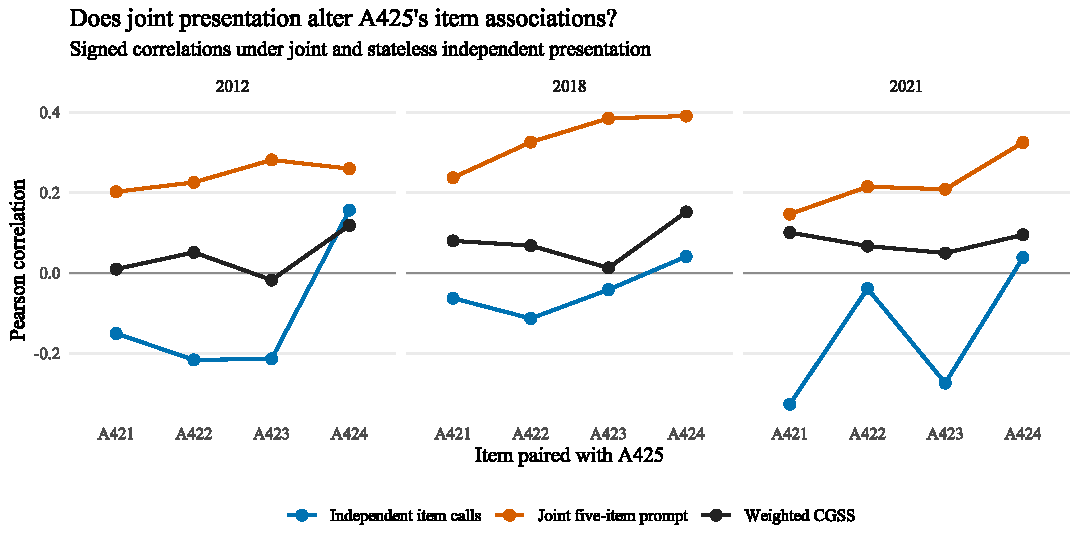
\includegraphics[width=\textwidth]{context_pair_correlations_en.pdf}
\caption{Signed A425 item correlations under joint and independent presentation. The joint series averages five repeat-specific correlations.}
\label{fig:context}
\end{figure}

\subsection{Sparse profiles do not explain the full gap}

\Cref{tab:matched} addresses the main alternative explanation. The supervised models are not highly accurate at the individual level: HGB's ordinal MAE is 0.921 and multinomial logit's is 0.935. Sparse demographics therefore impose a real information ceiling. Yet both recover aggregate distributions far better than Qwen3.5-9B. HGB's total variation is 0.071, compared with 0.282 for the LLM. Even the empirical marginal prior, which learns no mapping from profiles to attitudes, attains an MAE of 0.975 and total variation of 0.097.

\begin{table}[H]
\centering
\caption{Matched-profile predictive and distributional performance}
\label{tab:matched}
\begin{threeparttable}
\begin{tabular}{lrrrr}
\toprule
Model & Ordinal MAE & Abs. mean error & Total variation & Variance ratio \\
\midrule
Empirical marginal prior & 0.975 & 0.127 & 0.097 & 0.992 \\
Multinomial logit & 0.935 & 0.113 & 0.082 & 0.982 \\
Histogram gradient boosting & \textbf{0.921} & \textbf{0.093} & \textbf{0.071} & 0.986 \\
Stratified joint donor & 0.987 & -- & 0.070 & 0.973 \\
Qwen3.5-9B, zero-shot & 1.175 & 0.712 & 0.282 & 0.794 \\
\bottomrule
\end{tabular}
\begin{tablenotes}[flushleft]
\footnotesize
\item Notes: Models are evaluated on the same 300 CGSS profiles used for LLM generation. ML predictions are out of fold. The empirical marginal prior uses training-fold outcome frequencies but no profile attributes. ML variance uses the full predictive probability distribution; the Qwen3.5-9B row uses the empirical option distribution from five draws per profile.
\end{tablenotes}
\end{threeparttable}
\end{table}

\begin{figure}[H]
\centering
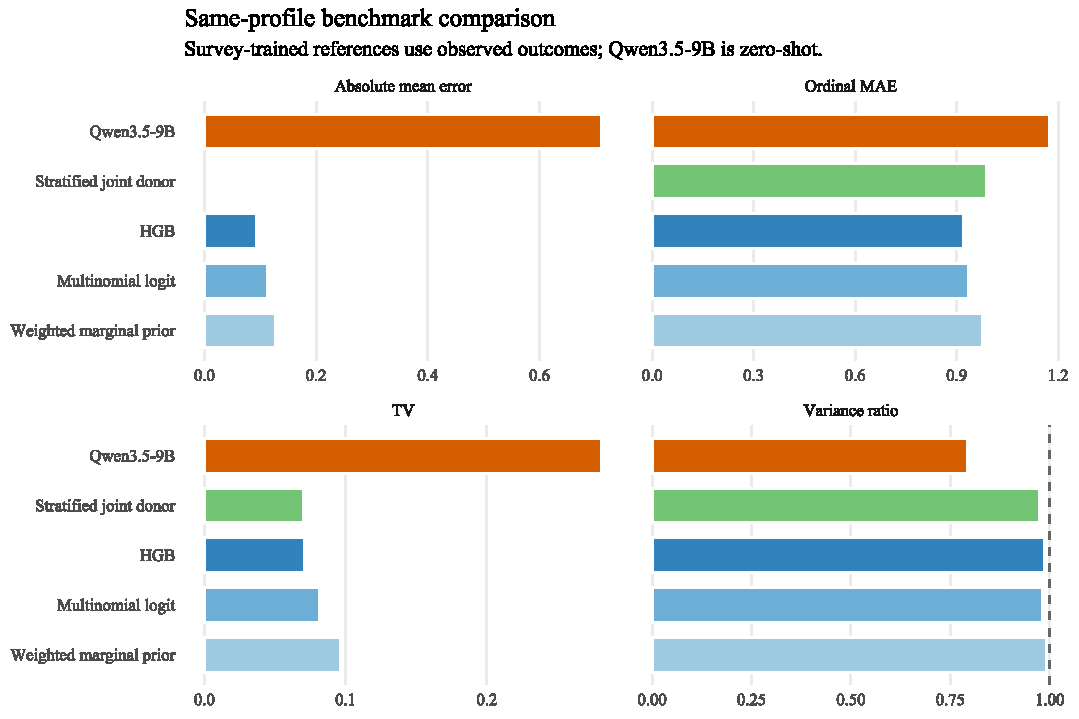
\includegraphics[width=\textwidth]{benchmark_comparison_en.pdf}
\caption{Same-profile comparison between survey-trained models and Qwen3.5-9B. Lower values indicate better performance. The absolute mean-error panel averages absolute cell-level mean errors rather than allowing positive and negative errors to cancel.}
\label{fig:model-comparison}
\end{figure}

The paired comparison is also precise within the matched sample. Qwen3.5-9B's absolute ordinal error exceeds HGB's by 0.255 points; the profile-cluster bootstrap interval is $[0.205,\,0.301]$. The five item errors belonging to one respondent are never treated as independent observations.

The joint donor supplies the relational counterpoint that item-wise classifiers cannot. Its correlation-matrix RMSE is 0.085 and its A425 mean absolute correlation is 0.105, compared with 0.173 and 0.270 for Qwen3.5-9B. Preserving complete human response vectors therefore recovers most of the joint structure without requiring a complex generator. This does not make the donor a zero-shot competitor; it demonstrates that sparse stratification does not mechanically require the excessive coherence produced by the LLM.

These findings do not establish that HGB is a superior model of human psychology. It is optimized on the outcomes being evaluated, while Qwen3.5-9B is not. Instead, they test a simpler account of the LLM results: that any method restricted to these demographic profiles must generate the same distorted population. Survey-trained models can remain uncertain about individuals while representing observed base rates and conditional variation more faithfully. Qwen3.5-9B adds a directionally patterned error beyond that limitation.

\subsection{Out-of-period prediction}

Random-fold comparisons allow the outcome-informed models to learn the marginal distribution of each survey year. A stricter test trains on 2012 and 2018 and predicts 2021. As \cref{tab:temporal} shows, every supervised reference deteriorates under temporal transfer. HGB's ordinal MAE rises to 0.942 on the matched 2021 profiles and its total variation rises to 0.107, indicating real distribution shift. This is substantively informative: even task-specific models cannot treat public opinion as time invariant.

\begin{table}[H]
\centering
\caption{Temporal generalization: train on 2012 and 2018, test on 2021}
\label{tab:temporal}
\begin{tabular}{lrrrr}
\toprule
Model & Ordinal MAE & RPS & Total variation & Variance ratio \\
\midrule
Historical marginal prior & 0.997 & 0.160 & 0.113 & 0.960 \\
Multinomial logit & 0.960 & 0.153 & 0.140 & 0.927 \\
Histogram gradient boosting & \textbf{0.942} & \textbf{0.150} & \textbf{0.107} & 0.955 \\
\bottomrule
\end{tabular}
\end{table}

On the 100 matched 2021 profiles, the historical references are compared with Qwen3.5-9B without allowing them to observe 2021 outcomes. This comparison still does not equalize training information---the references see historical CGSS labels---but it tests whether the LLM's 2021 fit is solely an artifact of allowing reference models to observe the target year's answers.

\section{Discussion}

\subsection{What the benchmark identifies}

The strongest inference is comparative. Demographic profiles provide limited information about any one person's gender attitudes. That limitation is visible in the residual MAE of the survey-trained models and is consistent with the modest explanatory power of standard demographic regressions. However, sparse profiles do not force a model to produce the particular population generated by Qwen3.5-9B. Outcome-informed references recover marginal distributions and matched answers more accurately. The language model's error therefore combines an information ceiling with additional model-specific or prompt-specific distortion.

This distinction matters for evaluating synthetic respondents. Individual prediction and population reconstruction are different estimands. Social scientists may tolerate low exact-match accuracy if a generator is calibrated and preserves the relationships required for inference. The Qwen3.5-9B case fails several parts of this more permissive population test: it shifts item means, weakly differentiates profiles, and strengthens relationships around a housework norm that is only weakly connected to the other items in CGSS.

The context experiment shows that prompt architecture is part of the data-generating process. Presenting the battery jointly increases positive item binding in the pooled audit, but the effect is not stable across waves and stateless calls create their own variance compression and negative associations. Independent prompting is therefore not an automatic correction. The defensible inference is that shared presentation amplifies an existing structural tendency; the remaining distortion may reflect model representations, item-specific decoding, or the changed output schema.

The comparison also clarifies what the marginal prior does and does not show. It does not constitute an unsupervised or information-free baseline; it uses observed outcome frequencies from training data. Its role is to separate personalization from base-rate calibration. If a non-personalized prior outperforms Qwen3.5-9B, the LLM's demographic conditioning does not compensate for its incorrect implicit base rates. It does not mean a prior can replace a survey, because those base rates must first be measured.

\subsection{Implications for gender-attitude research}

The substantive pattern is not a generic left- or right-leaning shift. Qwen3.5-9B overstates egalitarianism on the first four traditional statements, especially family orientation and male ability, while understating support for equal housework. A single ideological-bias label would therefore conceal the model's item-specific errors. The model also over-associates A425 with the other items, making human attitudes look more consistently ordered than they are.

This result returns to a central insight of multidimensional gender-ideology research: ambivalence can be socially meaningful. People can endorse equality in one setting and resist it in another. If synthetic respondents are optimized, prompted, or decoded in ways that favor internally consistent personas, they may erase precisely the combinations that social scientists seek to explain. Such data would be particularly hazardous for scale construction, latent-class analysis, subgroup inference, or simulations of attitude change.

\subsection{Limitations and next tests}

Five limitations define the scope of the current evidence. First, the audit evaluates one open-weight model. The findings should be described as a Qwen3.5-9B case study until replicated across model families and parameter scales. Second, five repeated draws provide an empirical option distribution but remain coarser than direct candidate-option probabilities. The resulting entropy and calibration diagnostics are therefore less precise than a logit-level audit. Third, the joint-versus-independent contrast changes not only item co-presence but also the structured-output schema, so it identifies a presentation bundle rather than an isolated context mechanism.

Fourth, prompt conditions are not fully factorial. The original, neutral, verbal-label, and paraphrased prompts change more than one feature at a time. They cannot separately identify the effects of social-desirability instructions, wording, and output format. A preregistered $2\times2$ design would provide a cleaner prompt-sensitivity test. Fifth, the survey battery itself is imperfect. A425 is a single positively worded item, whereas A421--A424 are traditional statements that are reverse-coded. The human benchmark establishes that unconditional aggregation is questionable, but it cannot separate domain content from all wording and measurement effects.

Two extensions are therefore more informative than adding further descriptive metrics. A factorial prompt experiment can separate item co-presence, conversation history, and output schema. A cross-model replication can determine whether the observed distortions are specific to Qwen3.5-9B or recur across model families. Perplexity and item-response models may be useful later, but neither substitutes for those identification tests.

\section{Conclusion}

Synthetic respondents should be evaluated as populations, not merely as fluent impersonations. In this study, a locally deployed Qwen3.5-9B model fails to reproduce several basic properties of Chinese gender attitudes. It generates large, item-specific mean errors, weak stable differentiation among profiles, and stronger coherence between the equal-housework item and the other gender-attitude items than appears in CGSS. Stateless item presentation reduces this coherence on average but does not recover the human structure consistently across waves.

The survey-trained benchmark changes the interpretation of that failure. Sparse demographic profiles do limit individual prediction, but models using the same prediction-time features can recover the observed distributions substantially better after outcome calibration. The LLM's distortion therefore cannot be reduced to missing profile information alone. At the same time, the comparison does not establish a universal defect of language models or identify a single mechanism. It establishes a narrower methodological point: claims about synthetic populations require benchmarks for base rates, heterogeneity, and covariance, together with explicit accounting of what each model observes during training and prediction.

\bibliographystyle{apalike}
\bibliography{references}

\end{document}
